\subsection{Proposed extension of the RDF provenance graph}
\label{sec:prov_rdf_extension}
In our analysis of CWLProv, described in the previous sections, we observed that much of the metadata was absent from the RDF representation of the execution. In this section, we describe the design and implementation of an extension to the provenance graph, in order to make more of the analysis accessible to exploration with SPARQL queries. 



Primarily, we aimed to expand the description of the workflow (i.e. \emph{prospective provenance}). Whereas the original design only mentioned the top-level workflow and its steps, the extended design incorporates all components for which the CWL Standards specify metadata fields (Table \ref{tab:metadata_fields}). In addition, provenance metadata supplied according to the annotation scheme described in the previous section is propagated to RDF. The details of the design are described in Supplementary Material (Section \emph{\nameref{sec:dev_recommendatons}}). 
% \stodor{explicitly where in the supplemental materials? with link}

We \stodor{TODO (Michael)} realized the extended design in the CWL reference implementation \emph{cwltool}. Repeating the analysis of CWLProv, we found that the extended RDF graph is notably richer in provenance metadata (Table \ref{tab:rdf_after}). Although still dependent on manual input from the workflow author, \textbf{Scientific context (\ref{tax:context})} is now fully represented in RDF, as well as \textbf{Data (\ref{tax:data})} and \textbf{Workflow (\ref{tax:wf})}. Future work should focus on the representation of workflow resource requirements, as well as computational environment. A list of SPARQL queries \stodor{TODO (Renske)} can be found in the Supplementary Material (Section \emph{\nameref{sup:sparql}}). 


\begin{table}[ht!]
\caption{RDF provenance graph after extension. The table shows for each taxonomy component whether it is fully (black) or partially represented (white), highlighting elements with improved representation in the extended design (\FiveStar). Components which are not represented in any of the documents are marked with an asterisk ($\ast$). Representations which are only included when this metadata is manually supplied are indicated with parentheses.}\label{tab:rdf_after}
% Use "S" column identifier (from siunitx) to align on decimal point.
% Use "L", "R" or "C" column identifier for auto-wrapping columns with tabularx.
% \todorenske{D2?}
% \todorenske{What about intermediate output data? Is there annotation for those possible? If not, shouldn't we change it to partial, instead of full representation?}
\begin{tabularx}{\linewidth}{l l L l }
\toprule
{Type} & {Subtype} & {Name} & {structured (RDF)} \\
\midrule
T1  & {SC1}  & Workflow design  & (\FiveStar)    \\
    & SC2   & Entity annotations                & (\FiveStar)     \\
    & SC3   & Workflow execution annotations   &  (\FiveStar)    \\
\midrule
T2  & D1    & Data identification               & (\FiveStar)     \\
    & D2    & File characteristics              & $\medsquare$ \\
    & D3    & Data access                       & (\FiveStar) \\
    & D4    & Parameter mapping                 & $\medblacksquare$  \\
\midrule
T3  & SW1   & Software identification           & ~  \\
    & SW2   & Software documentation            & ~ \\
    & SW3   & Software access                   & ~  \\
\midrule
T4  & WF1   & Workflow software metadata        & (\FiveStar) \\
    & WF2   & Workflow parameters               & (\FiveStar) \\
    & WF3   & Workflow requirements             & ~ \\
\midrule
T5  & ENV1  & Software environment $\ast$       & ~  \\
    & ENV2  & Hardware environment $\ast$       & ~ \\
    & ENV3  & Container image                   & $\medsquare$ \\
\midrule
T6  & EX1   & Execution timestamps              &  $\medblacksquare$\\
    & EX2   & Consumed resources                &  ~ \\
    & EX3   & Workflow engine                   & $\medsquare$ \\
    & EX4   & Human agent                       & $\medblacksquare$  \\
\bottomrule
\end{tabularx}


% \begin{tablenotes}
% \item Source is from this website: \url{https://www.sedl.org/afterschool/toolkits/science/pdf/ast_sci_data_tables_sample.pdf}
% \end{tablenotes}
\end{table}


%\begin{table}[bt!]
\caption{Metadata fields in CWL Standards v1.2. \emph{format} is only allowed for parameters of type File or File array.}\label{tab:metadata_fields}
\begin{tabularx}{\linewidth}{L l l l l}
\toprule
CWL field & Schema.org term \\
\midrule
% Widgets & 42 & Over-supplied\textsuperscript{*} \\
% Gadgets & 13 & Under-supplied \\
doc & description \\ %\hline
label & name \\ %\hline
format & encodingFormat \\
intent & featureList \\

\bottomrule
\end{tabularx}
\begin{tablenotes}
\item This is a table note.
\item \textsuperscript{*}Another note.
\end{tablenotes}
\end{table}


% \begin{figure*}[ht]
    \centering
    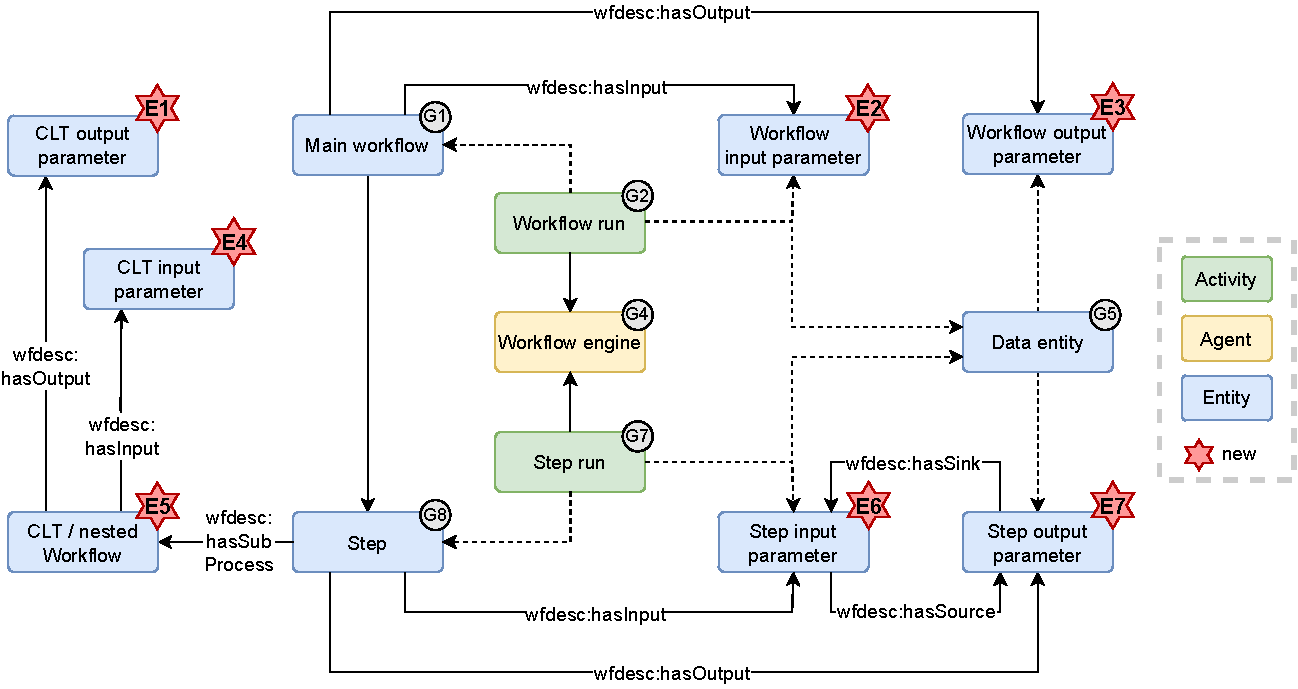
\includegraphics[width=0.99\textwidth]{rdf_extension/CWLProv_graph_extended.pdf}
    \caption{The RDF provenance graph, now extended with \emph{CommandLineTools} and parameter entities. Red stars mark nodes which are part of the design extension. Parameters are linked to their \emph{Workflow}, \emph{CommandLineTool} or step via \emph{wfdesc:hasInput} and \emph{wfdesc:hasOutput}. Node G5 represents both input and output data entities. The data flow between steps is represented via \emph{wfdesc:hasSink} and \emph{wfdesc:hasSource}. Steps are linked to their underlying tools via \emph{wfdesc:hasSubProcess}.}
    \label{fig:cwlprov_graph_new}
\end{figure*}



% \begin{figure}[ht]
    \centering
    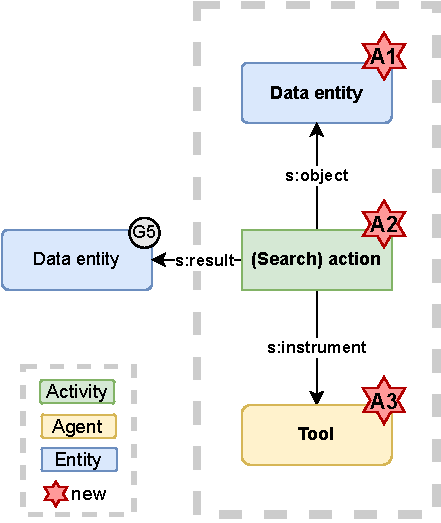
\includegraphics[width=0.4\textwidth]{rdf_extension/CWLProv_graph_extended_actions.pdf}
    \caption{Actions represented in RDF provenance graph. Workflow input datasets (\textbf{G5}) are connected to the Actions (\textbf{A2}) which produced them via \emph{s:result}. In addition, Actions can have properties such as \emph{object} (\textbf{A1}) and \emph{instrument} (\textbf{A3}).  }
    \label{fig:cwlprov_graph_actions}
\end{figure}